\documentclass{ctexart}
\usepackage{graphicx}
\begin{document}
我们把HPSP算法应用到自然语言的层次聚类问题。
一方面我们通过这个小例子展示HPSP在社群发现实际数据上的效果,
另一方面语言的分类对印欧语言研究较多,已有完善的标准。 
而对其他具体某一地区方言和少数民族语言研究较少,使用
算法自动聚类对于辅助语言学家在后者发力也有裨益 \cite{nasution2019visualizing}。

我们使用的数据是关于词汇相似率的数据。
词汇相似率是一个百分比,表示两种语言中有相同词意和书写方式的词汇比例
\cite{bella2021database}。
我们从Bella提供的数据中选取了67种常用语言,选取的标准是原
数据集中词汇相似率置信程度高且两两间均有相似率的语言。
在此基础上我们用 HPSP 算法进行聚类,得到了如下图所示的聚类树。
\begin{figure}[!ht]
    \centering
    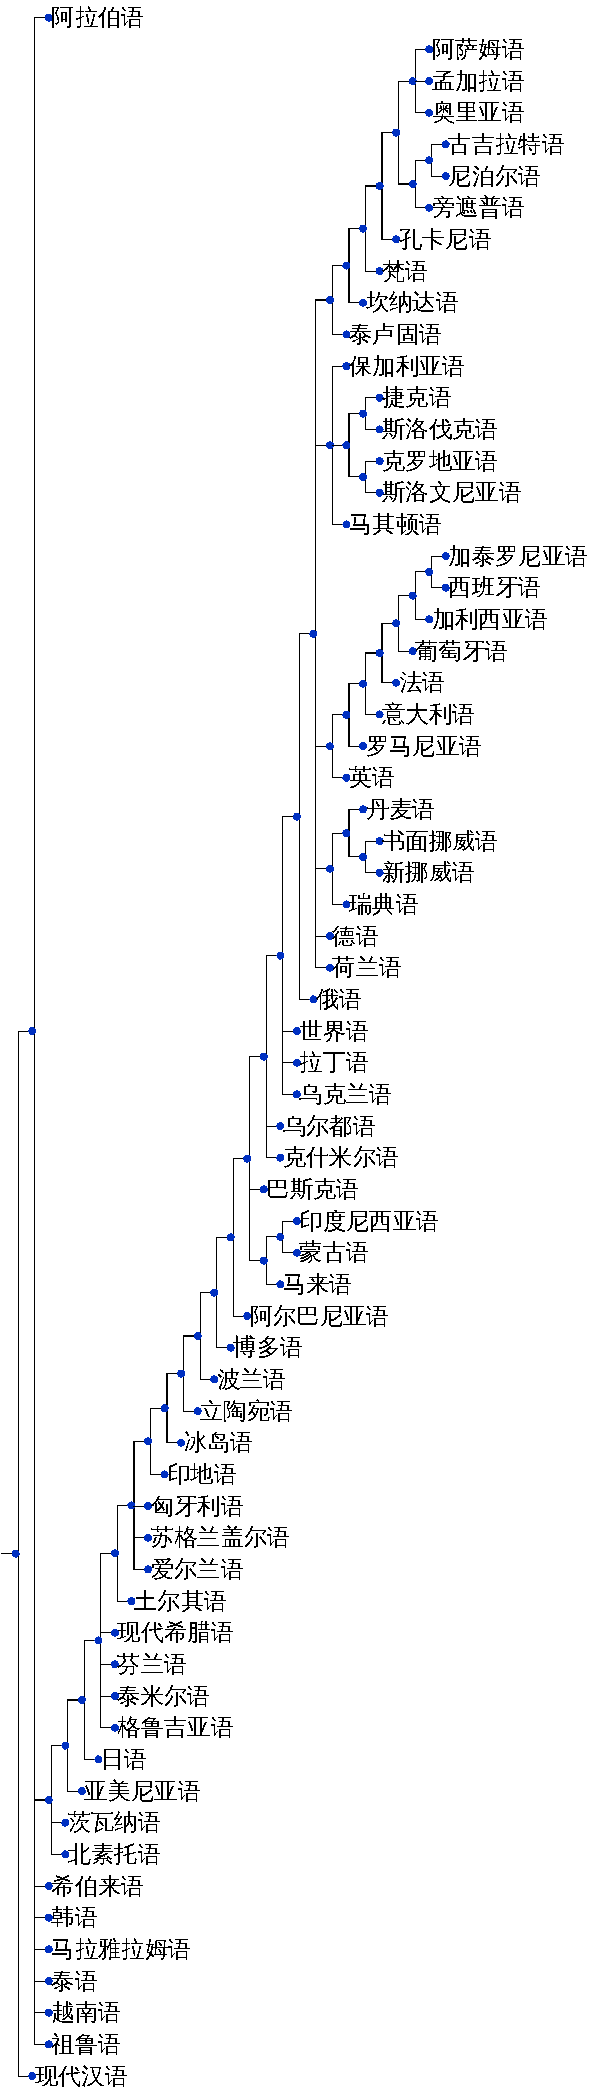
\includegraphics[width=\textwidth]{figures/language_tree.pdf}
    \caption{世界常用语言聚类树示意图}\label{fig:language_tree}
\end{figure}
    
从上图我们可以解读出一些与比较语言学的一致的结论,比如法语、西班牙语、葡萄牙语
等亲缘关系很近,在上图中亦反映出来。

\cite{al2017characterization} 用了普通的聚合聚类的方式对10种常用语言进行聚类,


\bibliographystyle{plain}
\bibliography{ref/refs.bib}

\end{document}
